\section{Main Theoretical Result}\label{sec:decoupled}
In this section, we proceed with the final step in extending the neural path theory to CNN and ResNet. As with \citetalias{ch2020neural}, we first describe the deep gated network (DGN) setup that decouples the NPFs and NPV, and follow it up with the main result that connects the NPK and the NTK in the DGN setting. 
\FloatBarrier
\begin{figure}[h]
\begin{minipage}{0.73\columnwidth}
\resizebox{\columnwidth}{!}{
\begin{tabular}{|l|l|}\hline
Feature Network & Value Network \\
$z^{\text{f}}_{x,\Tf}(\cdot,0) =x^{\text{f}}$ &$z^{\text{v}}_{x,\Tdgn}(\cdot,0) =x^{\text{v}}$ \\
$q^{\text{f}}_{x,\Tf}(\iout,l) =\ip{\Tf(\cdot,\iout,l), z^{\text{f}}_{x,\Tf}(\cdot,l-1)}$  & $q^{\text{v}}_{x,\Tdgn}(\iout,l) =\ip{\Tv(\cdot,\iout,l), z_{x,\Tv}(\cdot,l-1)} $\\
%$G^{\text{f}}_{x,\Tf}(\iout,l) = \mathbf{1}_{\{q^{\text{f}}_{x,\Tf}(\iout,l)>0\}}$ & -\\
$z^{\text{f}}_{x,\Tf}(\iout,l) =q^{\text{f}}_{x,\Tf}(\iout,l)\cdot G^{\text{f}}_{x,\Tf}(\iout,l)$&$\bm{z^{\text{v}}_{x,\Tdgn}(\iout,l) =q^{\text{v}}_{x,\Tdgn}(\iout,l)\cdot G^{\text{f}}_{x,\Tf}(\iout,l)}$\\
$\hat{y}^{\text{f}}_{\Tf}(x) = \ip{\Tf(\cdot,\iout, d), z^{\text{f}}_{x,\Tf}(\cdot,d-1)}$ & $\hat{y}_{\Tdgn}(x) = \ip{\Tv(\cdot,\iout, d), z^{\text{v}}_{x,\Tdgn}(\cdot,d-1)}$\\\hline
\multicolumn{2}{|l|}{Hard ReLU: $G^{\text{f}}_{x,\Tf}(\iout,l) = \mathbf{1}_{\{q^{\text{f}}_{x,\Tf}(\iout,l)>0\}}$ or Soft-ReLU: $G^{\text{f}}_{x,\Tf}(\iout,l) = \frac{1}{1+\exp(-\beta.q^{\text{f}}_{x,\Tf}(\iout,l))}$}\\\hline
%\multicolumn{2}{|l|}{Hard ReLU: $G^{\text{f}} = \mathbf{1}_{\{q^{\text{f}}>0\}}$ or Soft-ReLU: $G^{\text{f}} = \frac{1}{1+\exp(-\beta.q^{\text{f}})}$}\\\hline
\end{tabular}
}
\end{minipage}
\begin{minipage}{0.26\columnwidth}
\resizebox{\columnwidth}{!}{
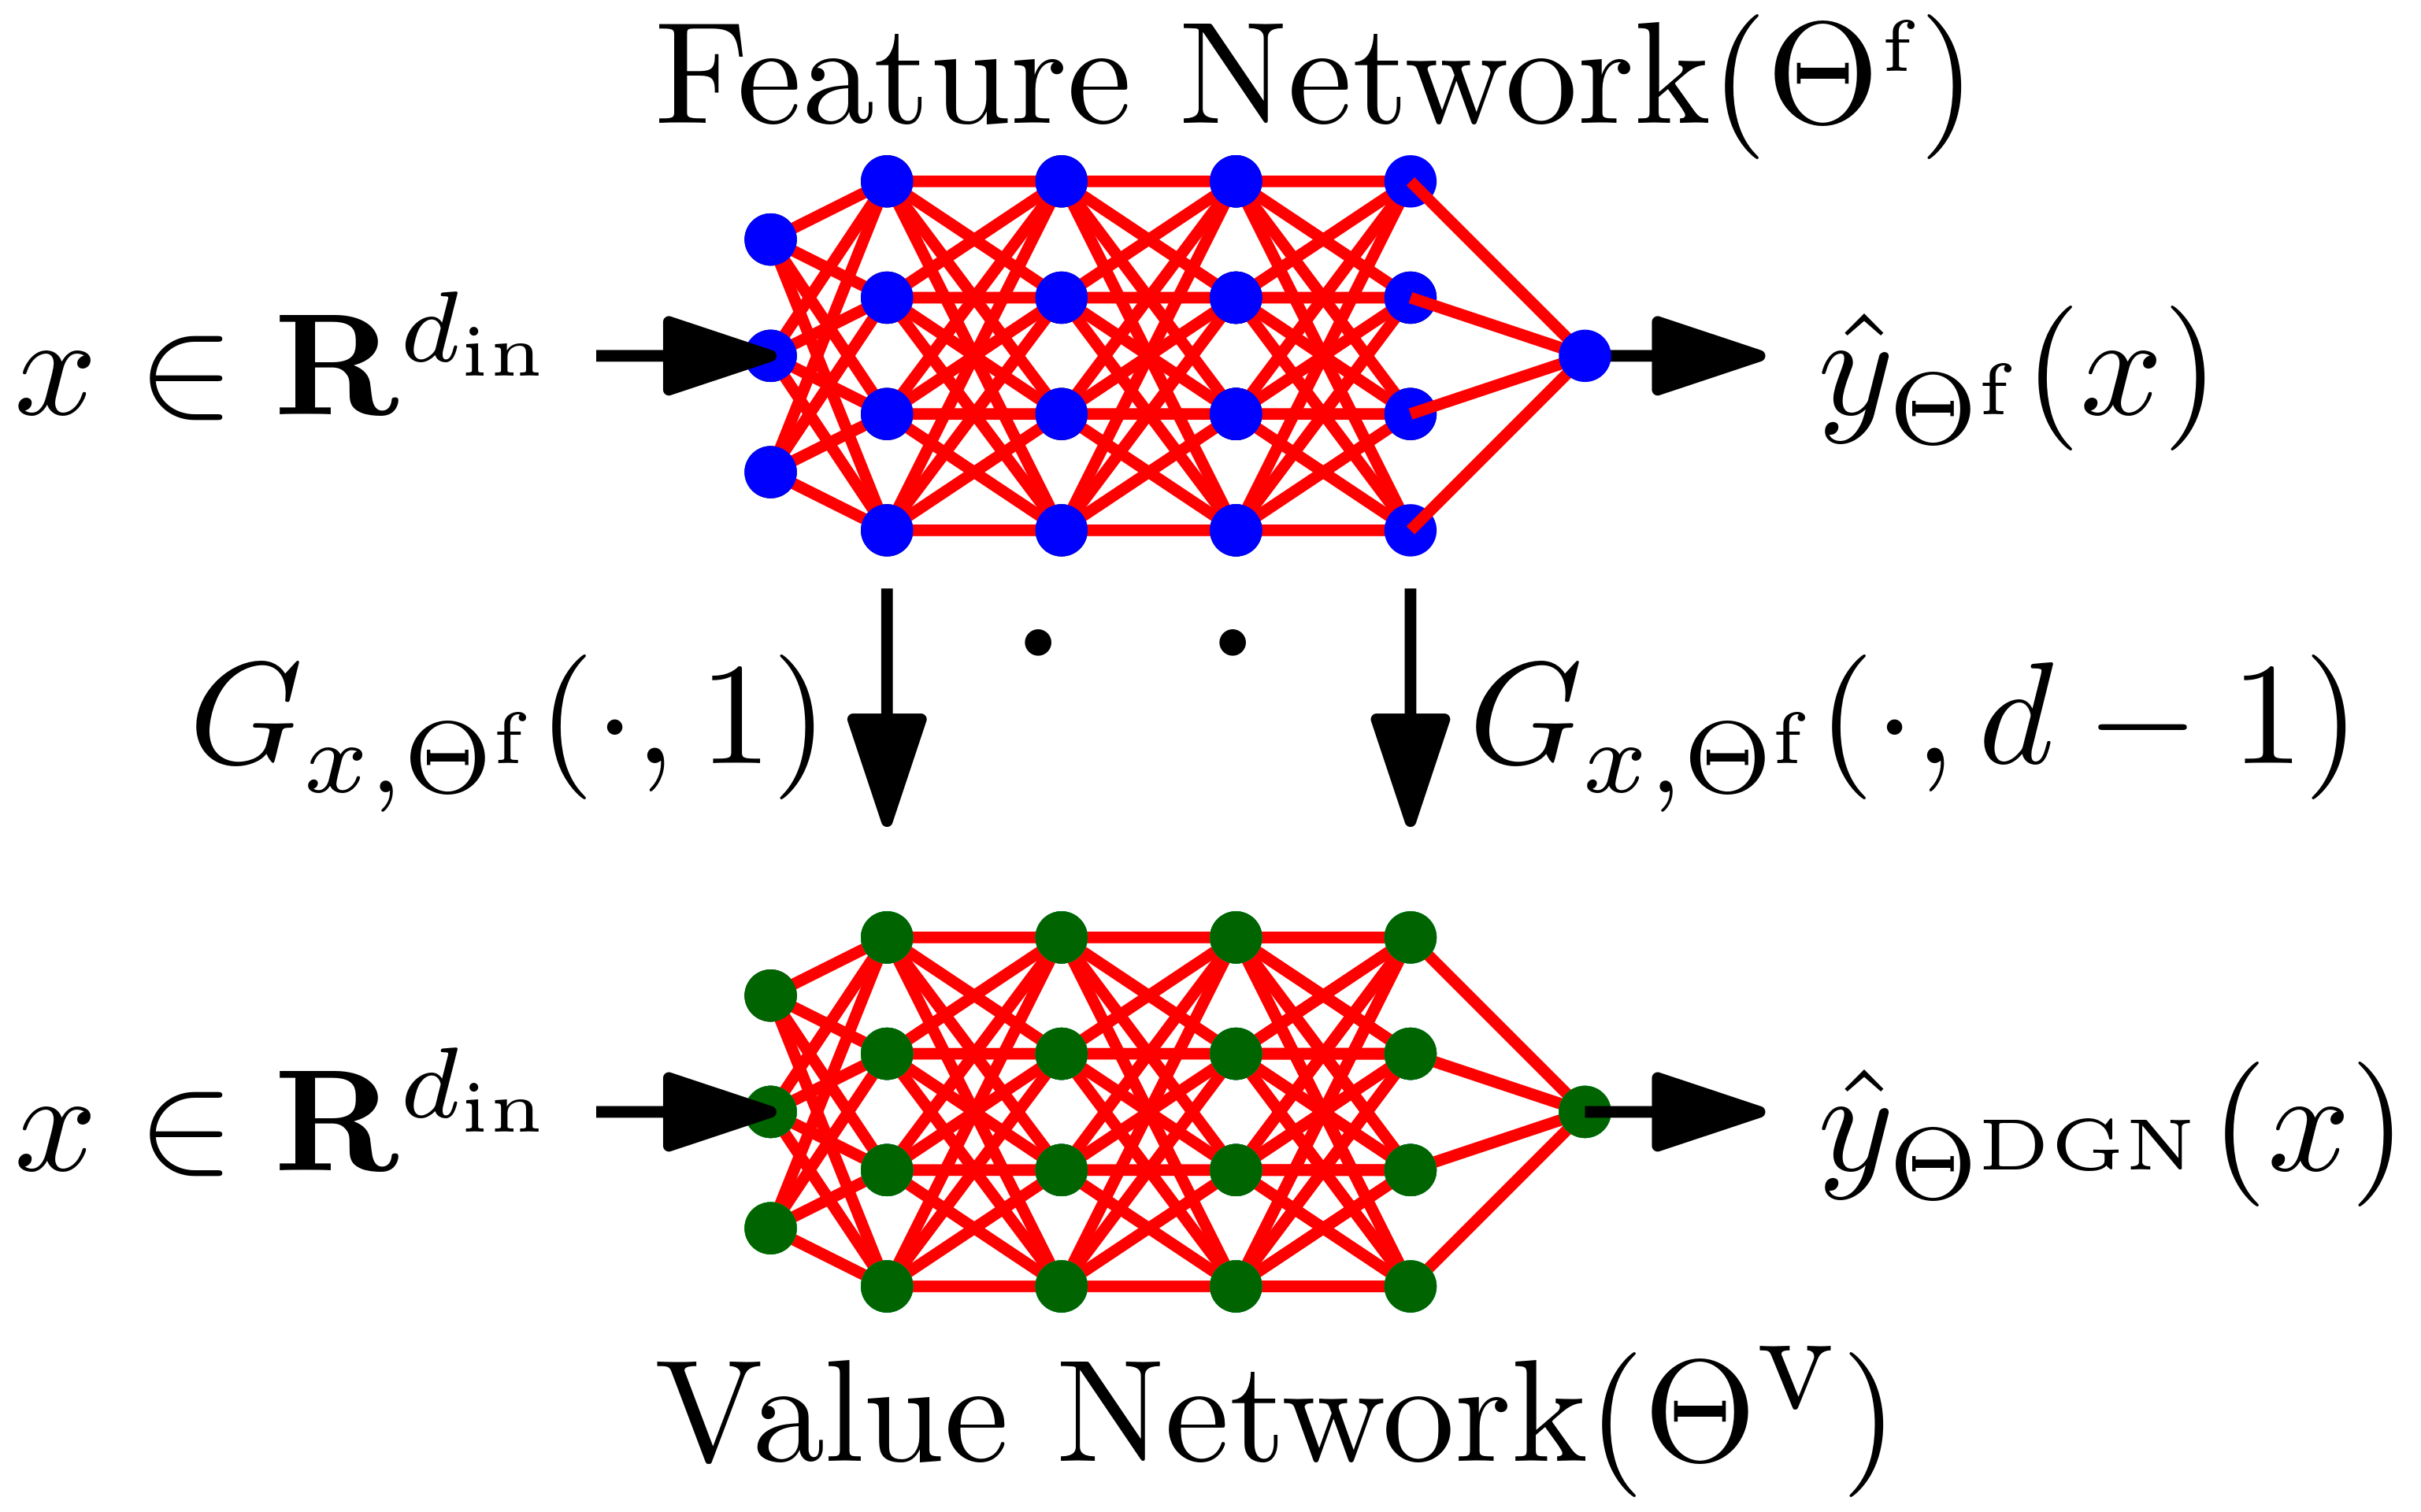
\includegraphics[scale=1]{figs/dgn-small.png}
}
\end{minipage}
\caption{\small{Shows a deep gated network (DGN). The soft-ReLU enables gradient flow into the feature network.}}
\label{fig:dgn}
\end{figure}

\textbf{DGN} set up was introduced by \citetalias{ch2020neural} to  analytically characterise the role played by the gates in a `standalone' manner. The DGN has two networks namely the \emph{feature network} parameterised by $\Tf\in\R^{d^{\text{f}}_{\text{net}}}$ which holds the NPFs (i.e., the gating information) and a \emph{value network} parameterised by $\Tv\in\R^{d^{\text{v}}_{\text{net}}}$ which holds the NPV.  The combined parameterisation is denoted by $\Theta^{\text{DGN}}=(\Tf,\Tv)\in \R^{d^{\text{f}}_{\text{net}}+d^{\text{v}}_{\text{net}}}$.  Thus the learning problem in the DGN is $\hat{y}_{\Tdgn}(x)=\ip{\phi_{x,\Tf},v_{\Tv}}$. 
% \subsection{Background: Deep Gated Networks}\label{sec:decoupled}
\begin{comment}
\begin{tabular}{lll}
Feature Network (FN) 	&:&	$\Tf\in\R^{\dfnet}$; provides the gates/masks i.e., the NPFs.\\
Value Network (VN)		&:&	$\Tv\in\R^{\dvnet}$; uses the gates/masks of FN to output $\hat{y}_{\Tdgn}(x)$.\\
Learning Problem &:& $\hat{y}_{\Tdgn}(x)=\ip{\phi_{x,\Tf},v_{\Tv}}$.
\end{tabular}
\end{comment}
\begin{comment}
\begin{wrapfigure}{r}{0.25\textwidth}
  \begin{center}
    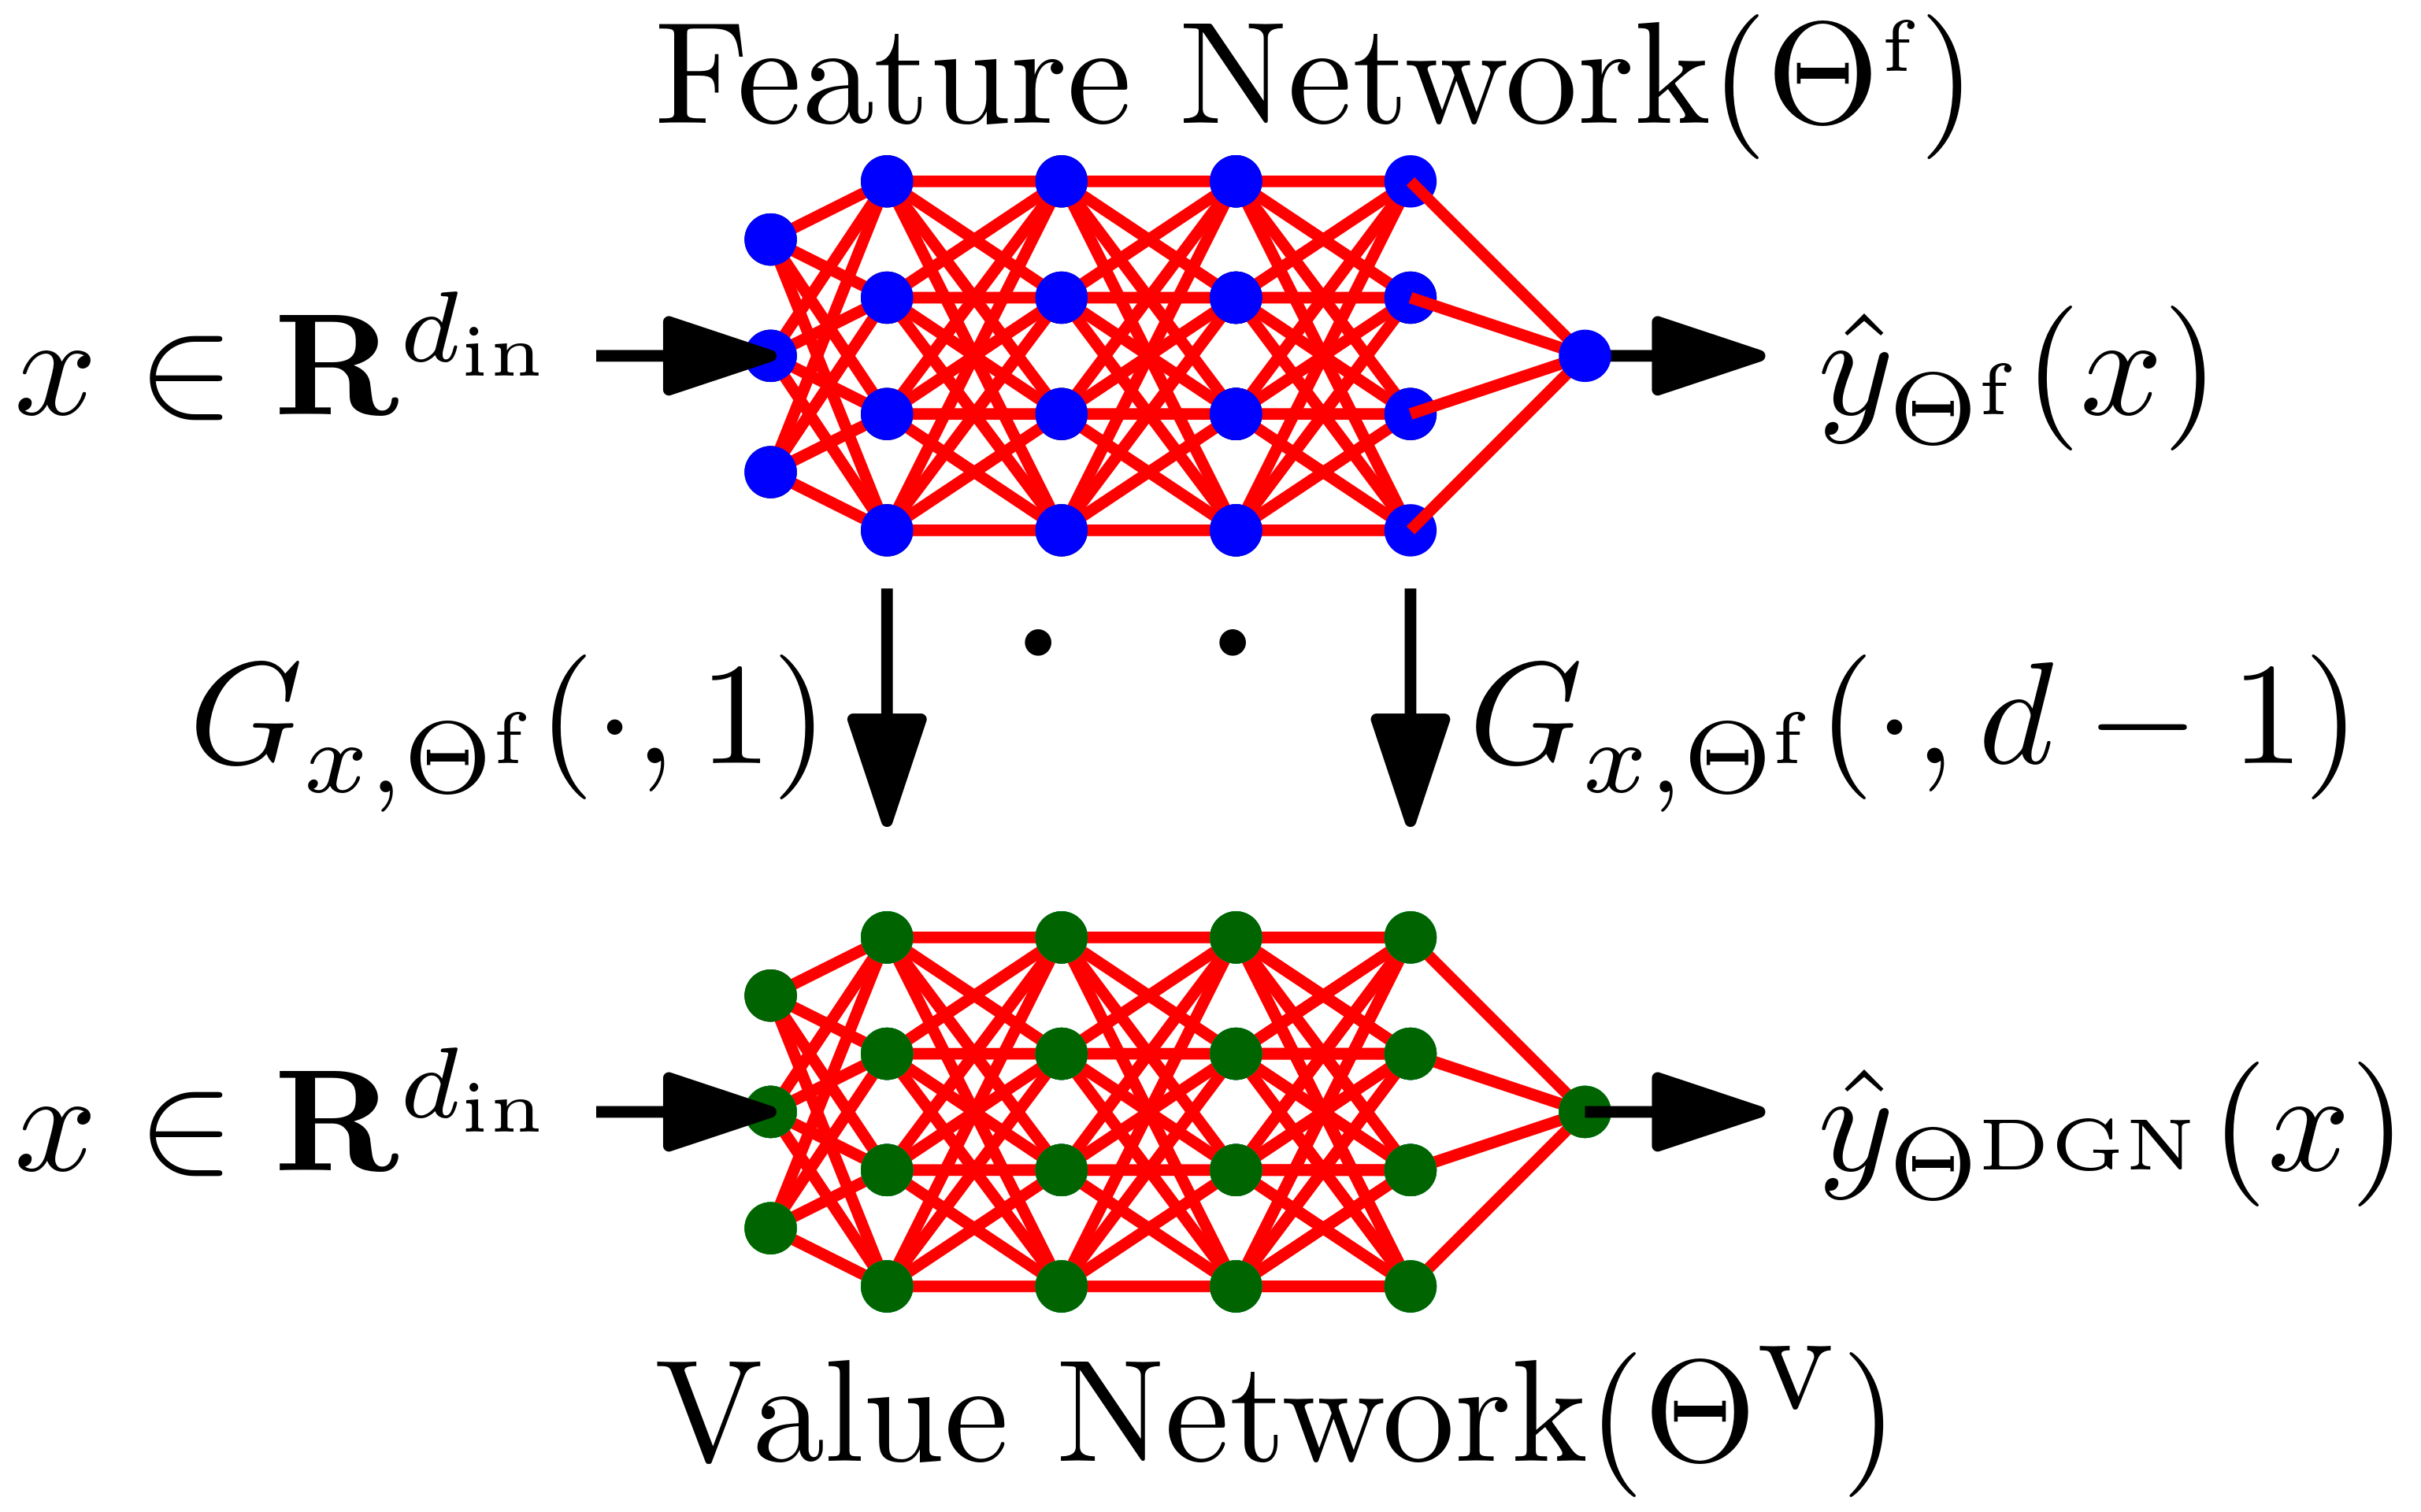
\includegraphics[width=0.25\textwidth]{figs/dgn-small.png}
  \end{center}
\caption{\small{DGN}}
\label{fig:dgn}
\end{wrapfigure}
\end{comment}
% Here the gates/`active sub-networks' are held in the feature network and are then used in the value network.
\begin{definition}\label{rm:regime}The DGN has $\mathbf{4}$ \textbf{regimes} namely \emph{decoupled learning} (DL), \emph{fixed learnt} (FL), \emph{fixed random-dependent initialisation} (FR-DI) and \emph{fixed random-independent initialisation} (FR-II). 
In all the regimes $\hat{y}_{\Tdgn}$ is the output, and $\Tv_0$ is always initialised at random and is \emph{trainable}. However, the regimes differ based on i) trainability of $\Tf$, ii) initialisation $\Tf_0$ as described below.\\
\begin{tabular}{lll}
DL              &: & $\Tf$ is trainable, and $\Tf_0$ and $\Tv_0$ are random and statistically independent,  $\beta>0$.\\
FL              &: & $\Tf$ is non-trainable, and $\Tf_0$ is pre-trained;  $\Tv_0$ is statistically independent of $\Tf_0$. \\
FR-II           &: & $\Tf$ is non-trainable, and $\Tf_0$ and $\Tv_0$ are random and statistically independent.\\
FR-DI   &:&  $\Tf$ is non-trainable, and $\Tf_0=\Tv_0$.\\
\end{tabular}
\end{definition}
\textbf{DGN Regimes:} The flexibility in a DGN is that  a) $\Tf$ can be trainable/non-trainable and b) $\Tf_0$ can be random or pre-trained using $\hat{y}_{\Tg}$ as the output (\Cref{rm:regime}). By using the DGN setup we can study the role of gates by comparing (a) learnable (DL) vs fixed gates (FL, FR-DI, FR-II), (b) random (FR-DI, FR-II) vs learnt gates (FL) and (c) dependent (FR-DI) vs independent initialisations (FR-II). In the DL regime `soft-ReLU' is chosen to enable gradient flow through the feature network.
%\end{comment}
\begin{comment}\textbf{Flattened Notation:} For a fully connected DNN of width $w$ and depth $d$, there are a total of $\ut=w(d-1)$ hidden units. Let  $q_{x,\Theta}(\iu)$, $G_{x,\Theta}(\iu)$, and $z_{x,\Theta}(\iu)$, where $\iu\in[\ut]$  denote the pre-activation, gating and output values of the $\ut$ hidden unit in the network, whose relationship is given in the left most illustration in \Cref{fig:hunit}.
\FloatBarrier
\begin{table}[h]
\resizebox{\columnwidth}{!}{
\begin{tabular}{|c|c|}\hline
Feature NTK & $\kv_{\Tdgn}(s,s')=\ip{\psiv_{x_s,\Tdgn},\psiv_{x_{s'},\Tdgn}}$, where $\psiv_{x,\Tdgn}=\nabla_{\Tv}\hat{y}_{\Tdgn}(x)\in\R^{\dvnet}$\\\hline
Value NTK & $\kf_{\Tdgn}(s,s')=\ip{\psif_{x_s,\Tdgn},\psif_{x_{s'},\Tdgn}}$, where $\psif_{x,\Tdgn}=\nabla_{\Tf}\hat{y}_{\Tdgn}(x)\in\R^{\dfnet}$\\\hline
\end{tabular}
}
\caption{Definition of NTF and NTKs for DGN used in \Cref{th:main}.}
\label{tb:defks}
\end{table}
\end{comment}

\begin{proposition}\label{prop:ntks} Let $K_{\Tdgn}$ be the NTK matrix of the DGN, then $K_{\Tdgn}=\kv_{\Tdgn}+\kf_{\Tdgn}$, with
%\FloatBarrier
\begin{table}[h]
\resizebox{\columnwidth}{!}{
\begin{tabular}{|c|c|}\hline
Overall NTK & $K_{\Tdgn}(s,s')=\ip{\psi_{x_s,\Tdgn},\psi_{x_{s'},\Tdgn}}$, where $\psi_{x,\Tdgn}=\nabla_{\Tdgn}\hat{y}_{\Tdgn}(x)\in\R^{\dnet}$\\\hline
Feature NTK & $\kv_{\Tdgn}(s,s')=\ip{\psiv_{x_s,\Tdgn},\psiv_{x_{s'},\Tdgn}}$, where $\psiv_{x,\Tdgn}=\nabla_{\Tv}\hat{y}_{\Tdgn}(x)\in\R^{\dvnet}$\\\hline
Value NTK & $\kf_{\Tdgn}(s,s')=\ip{\psif_{x_s,\Tdgn},\psif_{x_{s'},\Tdgn}}$, where $\psif_{x,\Tdgn}=\nabla_{\Tf}\hat{y}_{\Tdgn}(x)\in\R^{\dfnet}$\\\hline
\end{tabular}
}
\end{table}
\end{proposition}
\textbf{Remark:} There are two separate NTKs, each one corresponding to feature and value networks respectively. In the case of fixed regimes, $\kf=0$. 

\begin{comment}
\begin{definition}
(i) For an input $x\in\R^{d_{in}}$, define $\psif_{x,\Tdgn}=\nabla_{\Tf}\hat{y}_{\Tdgn}(x)\in\R^{\dfnet}$, and $\psiv_{x,\Tdgn}=\nabla_{\Tv}\hat{y}_{\Tdgn}(x)\in\R^{\dvnet}$.  
(ii) For  $s,s'\in[n]$ define $\kf_{\Tdgn}(s,s')=\ip{\psif_{x_s,\Tdgn},\psif_{x_{s'},\Tdgn}}$ and  $\kv_{\Tdgn}(s,s')=\ip{\psiv_{x_s,\Tdgn},\psiv_{x_{s'},\Tdgn}}$.
\end{definition} 
\end{comment}
\begin{comment}
\begin{theorem}\label{th:main} Assume (i) $\Tv_0\inrdnet$ is statistically independent of $\Tf_0$ (ii) $\Tv_0$ are i.i.d symmetric Bernoulli over $\{-\frac{\sigma}{\sqrt{w}},+\frac{\sigma}{\sqrt{w}}\}$. Then, it follows that\\
(i) $\E\left[\kv_{\Tdgn_0}\right]=d \left(\frac{\sigma^2}{w}\right)^{(d-1)} H_{\Tf_0}$, (ii) $\kv_{\Tdgn_0}\ra d \left(\frac{\sigma^2}{w}\right)^{(d-1)} H_{\Tf_0}$ as $w\ra\infty$.
\end{theorem}
\end{comment}
\begin{comment}
\begin{assumption}\label{assmp:main}
(i) $\Tv_0$ is statistically independent of $\Tf_0$ (ii) $\Tv_0$ are sampled i.i.d from symmetric Bernoulli over $\{-{\sigma},+{\sigma}\}$. For FC layers $\sigfc=\frac{\cscale}{\sqrt{w}}$, and for convolutional layers $\sigcnn=\frac{\cscale}{\sqrt{w\wconv}}$.
\end{assumption}
\end{comment}
\begin{comment}
\begin{definition}[Scaling Factors]
For $\J\in 2^{[b]}$, define $\gamma_{\text{res}}(\J)=\underset{j\in \J}\Pi \gamma^{\text{pre}}_j \cdot \underset{j'\in [b]\setminus \J}\Pi \gamma^{\text{post}}_{j'}$, $\bfc=d\cdot\sigfc^{2(d-1)}$, $\bcnn=\frac{1}{{\din}^2} (\dconv \sigcnn^{2(\dconv-1)}\sigfc^{2\dfc}+\dfc \sigcnn^{2\dconv}\sigfc^{2(\dfc-1)}$, $\bres(\J)= (|\J| +2)\dblock \sigfc^{2( (|J|+2)\dblock-1)}$.
\end{definition}
\end{comment}
\begin{comment}
\begin{theorem}\label{th:main} (i) $\Tv_0$ is statistically independent of $\Tf_0$ (ii) $\Tv_0$ are i.i.d symmetric Bernoulli over $\{-{\sigma},+{\sigma}\}$. For FC layers $\sigfc=\frac{\cscale}{\sqrt{w}}$, and for convolutional layers $\sigcnn=\frac{\cscale}{\sqrt{w\wconv}}$. As $w\ra\infty$, it follows that: 
(i) FC: $\kv_{\Tdgn_0}\ra \bfc H_{\Tf_0}$,  (ii) CNN: $\kv_{\Tdgn_0}\ra \bcnn H_{\Tf_0}$, (iii) ResNet: $\kv_{\Tdgn_0}\ra \sum_{\J\in 2^{[b]}}  \bres^{\J} H^{\J}_{\Tf_0}$, where
\resizebox{\columnwidth}{!}{
\begin{tabular}{|c|c|c|}\hline
$\bfc$& $\bcnn$&$\bres^{\J}$ \\\hline
$d\sigfc^{2(d-1)}$  & $\frac{1}{{\din}^2} \left(\dconv \sigcnn^{2(\dconv-1)}\sigfc^{2\dfc}+\dfc \sigcnn^{2\dconv}\sigfc^{2(\dfc-1)}\right)$  &$(|\J| +2)\dblock \sigfc^{2\big( (|\J|+2)\dblock-1\big)} \left(\underset{j\in \J}\Pi \gamma^{\text{pre}}_j \cdot \underset{j'\in [b]\setminus \J}\Pi \gamma^{\text{post}}_{j'}\right)^2$\\\hline
\end{tabular}
}
\end{theorem}
\end{comment}
\begin{theorem}\label{th:main} (i) $\Tv_0$ is statistically independent of $\Tf_0$ (ii) $\Tv_0$ are i.i.d symmetric Bernoulli over $\{-{\sigma},+{\sigma}\}$. Let $\sigfc=\frac{\cscale}{\sqrt{w}}$ and $\sigcnn=\frac{\cscale}{\sqrt{w\wconv}}$ for FC and convolutional layers. As $w\ra\infty$, we have: 

(ii) $\kv_{\Tdgn_0}\ra \bfc H_{\Tf_0}$, $\bfc =d \sigfc^{2(d-1)}$ for FC-DNN,

(ii) $\kv_{\Tdgn_0}\ra \bcnn H_{\Tf_0}$, $\bcnn = \frac{1}{{\din}^2} \left(\dconv \sigcnn^{2(\dconv-1)}\sigfc^{2\dfc}+\dfc \sigcnn^{2\dconv}\sigfc^{2(\dfc-1)}\right)$ for  CNN with GAP,

(iii) $\kv_{\Tdgn_0}\ra \sum_{\J\in 2^{[b]}}  \bres^{\J} H^{\J}_{\Tf_0}$, $\bres^{\J} = (|\J| +2)\dblock \sigfc^{2\big( (|\J|+2)\dblock-1\big)} \Gamma(\J)^2$ for ResNet.
%\begin{align*}
%\bcnn &= \frac{1}{{\din}^2} \left(\dconv \sigcnn^{2(\dconv-1)}\sigfc^{2\dfc}+\dfc \sigcnn^{2\dconv}\sigfc^{2(\dfc-1)}\right)\\
%\bres^{\J} &= (|\J| +2)\dblock \sigfc^{2\big( (|\J|+2)\dblock-1\big)} \left(\underset{j\in \J}\Pi \gamma^{\text{pre}}_j \cdot \underset{j'\in [b]\setminus \J}\Pi \gamma^{\text{post}}_{j'}\right)^2
%\end{align*}
\end{theorem}

$\bullet$ $\bm{\bfc,\bcnn,\bres:}$ The simplest of all is $\bfc=d\sigfc^{2(d-1)}$, where $d$ is  due the fact that there are $d$ weights in a path and in the exponent of $\sigfc$, factor $(d-1)$ arises because the gradient of a particular weight is product of all the weights in the path excluding the said weight itself, and the factor of $2$ is due to the fact that NTK is an inner product of two gradients. $\bcnn$ is similar to $\bfc$ with separate bookkeeping for the convolutional and FC layers, and $\frac{1}{\din^2}$ is due to the GAP layer. In $\bres$, the $\bfc$ for all the sub-FC-DNNs within the ResNet are scaled by the corresponding normalisation factors and summed.

%$\bullet$ $\bm{\kf}$ vs $\bm{\kv}$: T
$\bullet$ \textbf{Decoupling} In a DNN with ReLU (and FR-DI regime of DGN), NPV and NPF are not statistically independent at initialisation, i.e., \Cref{th:main} does not hold. However, the current state-of-the-art analysis \cite{ntk,arora2019exact,cao2019generalization} is in the \emph{infinite width} ($w\rightarrow\infty$) regime, wherein, the change in activations during training is  only of the order $\sqrt{\frac{1}{w}}$, which goes to $0$ as $w\ra\infty$. Hence, though assumption in \Cref{th:main} may not hold exactly, it is \emph{not a strong assumption} to fix the NPFs for the purpose of analysis. Once the NPFs are fixed, it only natural to statistically decouple the NPV from fixed NPFs (\Cref{th:main} hold in FR-II, FL and DL regimes).  %Furthermore, \Cref{assmp:main} adds strength, it brings out the relationship  NTK = constant $\times$ NPK (in \Cref{th:main}). 

$\bullet$ \textbf{Gates are Key:} In simple terms, \Cref{th:main} says that if the gates/masks are known, then the weights are expendable, a fact which we also verify in our extensive experiments.
\begin{comment}
$\bullet$ \textbf{Base Kernel:} %We now informally reason out the behaviour of the base kernel $H^{\text{lyr}}_{l,\Theta_0}$ as a function of $l$. 
For each $l$, $H^{\text{lyr}}_{l,\Theta_0}$ is an inner product of the binary features, which at randomised initialisation, for infinite width is proportional $\frac{1}2-\frac{\text{arccos}\ip{z_{x_s,\Theta_0}(\cdot,l-1),z_{x_{s'},\Theta_0}(\cdot,l-1)}}{2\pi}$. Further, due to the property of ReLU to pass only positive components, it is likely that the angle $\ip{z_{x_s,\Theta_0}(\cdot,l-1),z_{x_{s'},\Theta_0}(\cdot,l-1)}$ keeps reducing with depth and $\frac{H^{\text{lyr}}_{l,\Theta_0}(s,s')}{w}\ra\frac{1}{2},\forall s,s'\in[n]$. 
\end{comment}
\begin{comment}
$\bullet$ \textbf{Interpretability:} \Cref{th:main} shows that the gates and the active sub-networks are \emph{fundamental entities arising naturally in the NTK framework}. The NPK is \emph{interpretable} in terms of the gates and active sub-networks, while NTK is defined in terms of gradients with no such interpretation. Further,\\
\indent \quad $1.$ The role of depth is interpretable in terms of the relation between $H^{\text{fc}}$ and $H^{\text{lyr}}$, and the role of residual connections,  as well as convolutions is capture in the structure of the NPK (see \Cref{sec:npk}).\\
\indent \quad $2.$ In the light of the result in \Cref{th:main} deep learning can be interpreted as a \emph{multiple kernel learning} method. Our experiments do suggest a strong evidence that the NPKs are learnt.
\end{comment}
\begin{comment}
$\bullet$ \textbf{Finite Width:} The $w\ra\infty$ condition in \Cref{th:main} needs to hold only for the value network. For the feature network, $w\ra\infty$ instead can be achieved by copying the gates of such a DNN into the feature network of identical architecture, and repeating it $m$ times and letting $m\ra\infty$ instead. 
\end{comment}
%$\bullet$ An extension of \Cref{th:main} to ResNets and CNNs is in the appendix.





